\documentclass[11pt]{article}
\usepackage[utf8]{inputenc}
\usepackage[T1]{fontenc}
\usepackage{amsmath}
\usepackage{amssymb} % Needed for \eth if used
\usepackage{graphicx}
\usepackage{geometry}
\usepackage{tikz}
\usepackage{pgfplots} % For plots
\usepackage{ulem}     % For underline, using normalem to avoid messing with \emph
\usepackage{booktabs} % For better tables
\usepackage{tcolorbox} % For boxing equations if needed
\usepackage{braket}    % For QM state notation if needed

\geometry{a4paper, margin=1in}
\usetikzlibrary{positioning, arrows.meta, shapes.geometric, patterns, calc} % Added calc library
\pgfplotsset{compat=1.18} % Use a recent PGFPlots version

% Custom commands (optional)
\newcommand{\avg}[1]{\overline{#1}}
\newcommand{\prob}[1]{P(#1)}
\newcommand{\ProbDens}[1]{\mathcal{P}(#1)} % Using script P for density
\newcommand{\vect}[1]{\vec{#1}}
\newcommand{\dd}[1]{\mathrm{d}#1} % Differential d
\newcommand{\pderiv}[2]{\frac{\partial #1}{\partial #2}}
\newcommand{\deriv}[2]{\frac{\mathrm{d} #1}{\mathrm{d} #2}}
\newcommand{\muState}{\mu\text{-state}} % Microstate
\newcommand{\OmegaE}{\Omega(E)}
\newcommand{\omegaE}{\omega(E)}
\newcommand{\PhiE}{\Phi(E)}
\newcommand{\deltaE}{\delta E}
\newcommand{\ethbar}{\text{\it{đ}}} % \eth symbol for inexact differential
\newcommand{\kb}{k_B} % Boltzmann constant
\newcommand{\gasR}{R} % Ideal gas constant
\newcommand{\partfn}{Z} % Partition function symbol
\newcommand{\grandpartfn}{\mathcal{Z}} % Grand partition function symbol (using Z from source)
\newcommand{\eps}{\epsilon}

\title{Physics 415 - Lecture 27}
\date{March 31, 2025}
\author{} % Author not specified

\begin{document}

\maketitle
\thispagestyle{empty} % No page number on title page

\section*{Summary}

\subsection*{Canonical Ensemble (CE)}
\begin{itemize}
    \item Fixed $T, N, V$.
    \item Probability of microstate $r$: $P_r = \frac{e^{-\beta E_r}}{\partfn}$, where $\beta = 1/T$ ($T$ in energy units).
    \item Partition function: $\partfn = \sum_r e^{-\beta E_r}$.
    \item Energy $E$ fluctuates.
    \item Helmholtz Free Energy: $F = -T \ln \partfn$.
\end{itemize}

\subsection*{Grand Canonical Ensemble (GCE)}
\begin{itemize}
    \item Fixed $T, \mu, V$. ($\mu$ = chemical potential).
    \item Probability of microstate $r$ (with $N_r$ particles): $P_r = \frac{e^{-\beta(E_r - \mu N_r)}}{\grandpartfn}$.
    \item Grand partition function: $\grandpartfn = \sum_r e^{-\beta(E_r - \mu N_r)} = \sum_N e^{\beta \mu N} Z_N$.
    ($Z_N$ = N-particle canonical partition function).
    \item Grand Potential: $\Phi = -T \ln \grandpartfn$.
    \item Mean particle number: $\avg{N} = -\left( \pderiv{\Phi}{\mu} \right)_{T,V}$.
\end{itemize}

\section*{Quantum Statistical Mechanics of Ideal Gases}

Investigate statistical mechanics of systems at low T, where QM effects play an especially important role.
\begin{itemize}
    \item New effects are associated with "exchange statistics" of identical particles. We will have to consider identical particles.
    \item Discussion will be restricted to non-interacting particles ("ideal gas").
    \item As we will see, even in the absence of direct interaction forces, the effect of exchange statistics leads to a mutual coupling of particles.
\end{itemize}

\section*{Example: Two Particles in a 1D Box}

Before going into detailed formalism, we start with simple examples.
Consider a 1D box of length L with infinite potential walls.

\begin{center}
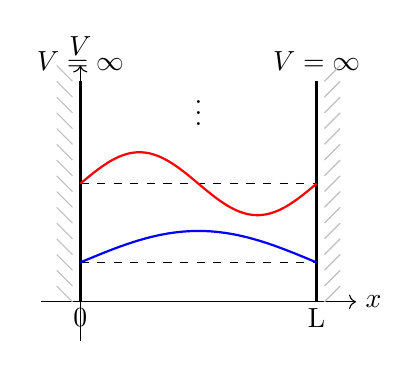
\begin{tikzpicture}
    % Axes
    \draw [->] (-0.5,0) -- (3.5,0) node [right] {$x$};
    \draw [->] (0,-0.5) -- (0,3) node [above] {$V$};

    % Walls
    \draw [very thick] (0,0) -- (0,2.8) node [above] {$V=\infty$};
    \draw [very thick] (3,0) -- (3,2.8) node [above] {$V=\infty$};

    % Box base and labels
    \draw (0,0) -- (3,0);
    \node at (0,-0.2) {0};
    \node at (3,-0.2) {L};

    % Energy levels (schematic) & Wavefunctions
    \draw [dashed] (0, 0.5) -- (3, 0.5); % n=1 level
    \draw[blue, thick] plot[smooth, domain=0:3] (\x, {0.5 + 0.4*sin(deg(\x*pi/3))});
    \draw [dashed] (0, 1.5) -- (3, 1.5); % n=2 level
    \draw[red, thick] plot[smooth, domain=0:3] (\x, {1.5 + 0.4*sin(deg(\x*2*pi/3))});
    \node at (1.5, 2.5) {$\vdots$};

    % Optional hatching for walls
    \foreach \y in {0, 0.2,...,2.8} {
        \draw[gray!50] (-0.1,\y) -- (-0.3, \y+0.2);
        \draw[gray!50] (3.1,\y) -- (3.3, \y+0.2);
    }
\end{tikzpicture}
\end{center}

Start w/ distinguishable particles, labelled "A" \& "B".
\begin{itemize}
    \item Hamiltonian: $H = H_A + H_B$, where $H_{A/B} = -\frac{\hbar^2}{2m} \frac{d^2}{dx_{A/B}^2}$.
    \item Schrödinger equation: $H \Psi(x_A, x_B) = E \Psi(x_A, x_B)$.
    \item Since particles are non-interacting, total energy is a sum of individual energies: $E_{rs} = \eps_r^{(A)} + \eps_s^{(B)}$.
    \item Single-particle energy levels: $\eps_r = \frac{\hbar^2}{2m} \left( \frac{\pi r}{L} \right)^2$, $r=1, 2, 3, \dots$. Same for $\eps_s$.
    \item The wave function is $\Psi_{rs}(x_A, x_B) = \varphi_r(x_A) \varphi_s(x_B)$ with $\varphi_r(x) \propto \sin\left(\frac{\pi r x}{L}\right)$.
\end{itemize}

\textbf{Picture Example:} ($r=2, s=3$)
\begin{center}
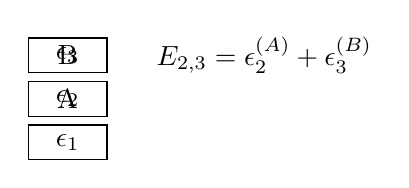
\begin{tikzpicture}[level/.style={draw, minimum width=1cm, minimum height=0.2cm}]
    \node[level] (e1) at (0,0) {$\eps_1$};
    \node[level] (e2) [above=0.1cm of e1] {$\eps_2$};
    \node[level] (e3) [above=0.1cm of e2] {$\eps_3$};
    \node at (e2.center) {A};
    \node at (e3.center) {B};
    \node[right=0.5cm of e3] {$E_{2,3} = \eps_2^{(A)} + \eps_3^{(B)}$};
\end{tikzpicture}
\end{center}

Now suppose particles A \& B are indistinguishable. States that were distinct become equivalent.
\textbf{Example:}
\begin{center}
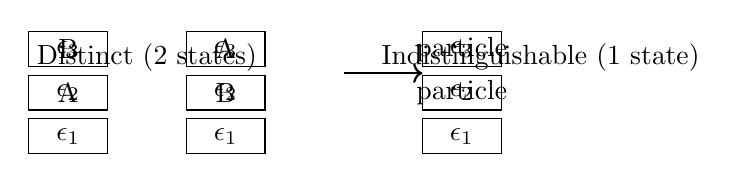
\begin{tikzpicture}[level/.style={draw, minimum width=1cm, minimum height=0.2cm}]
    % State 1
    \node[level] (e1a) at (0,0) {$\eps_1$};
    \node[level] (e2a) [above=0.1cm of e1a] {$\eps_2$};
    \node[level] (e3a) [above=0.1cm of e2a] {$\eps_3$};
    \node at (e2a.center) {A};
    \node at (e3a.center) {B};
    % State 2
    \node[level] (e1b) at (2,0) {$\eps_1$};
    \node[level] (e2b) [above=0.1cm of e1b] {$\eps_2$};
    \node[level] (e3b) [above=0.1cm of e2b] {$\eps_3$};
    \node at (e2b.center) {B};
    \node at (e3b.center) {A};
    \node at (1, 1) {Distinct (2 states)};

    % State 3 (Indistinguishable)
    \node[level] (e1c) at (5,0) {$\eps_1$};
    \node[level] (e2c) [above=0.1cm of e1c] {$\eps_2$};
    \node[level] (e3c) [above=0.1cm of e2c] {$\eps_3$};
    \node at (e2c.center) {particle};
    \node at (e3c.center) {particle};
    \node at (6, 1) {Indistinguishable (1 state)};
    \draw[->, thick] (3.5, 0.8) -- (4.5, 0.8); % Arrow between concepts
\end{tikzpicture}
\end{center}

\subsection*{Wave Functions for Identical Particles}

In terms of wave functions, we continue to use labels A \& B, but now we impose a symmetry requirement on the wave function under "exchange" of particles ($x_A \leftrightarrow x_B$). There are two cases:

\subsubsection*{Bose-Einstein Statistics (BE)}
\begin{itemize}
    \item Wave function is \uline{symmetric} under exchange: $\Psi_{rs}(x_A, x_B) = +\Psi_{rs}(x_B, x_A)$.
    \item Form: $\Psi_{rs}(x_A, x_B) \propto \varphi_r(x_A) \varphi_s(x_B) + \varphi_r(x_B) \varphi_s(x_A)$.
    \item Particles with symmetric wave functions have integer spin ($S=0, \hbar, 2\hbar, \dots$) and are called "bosons".
    \item Examples: photons, Higgs particle, $^4$He atoms, ...
\end{itemize}

\subsubsection*{Fermi-Dirac Statistics (FD)}
\begin{itemize}
    \item Wave function is \uline{antisymmetric} under exchange: $\Psi_{rs}(x_A, x_B) = -\Psi_{rs}(x_B, x_A)$.
    \item Form: $\Psi_{rs}(x_A, x_B) \propto \varphi_r(x_A) \varphi_s(x_B) - \varphi_r(x_B) \varphi_s(x_A)$.
    \item Particles with antisymmetric wave functions have half-integer spin ($S=\frac{\hbar}{2}, \frac{3\hbar}{2}, \dots$) and are called "fermions".
    \item Examples: $e^-$, protons/neutrons, $^3$He atoms, ...
    \item Suppose $r=s$: $\Psi_{rr}(x_A, x_B) \propto \varphi_r(x_A) \varphi_r(x_B) - \varphi_r(x_B) \varphi_r(x_A) = 0$.
    \item A given state may not be occupied by more than one identical fermion. This is the "\textbf{Pauli exclusion principle}".
    \item Note that no similar restriction applies for bosons (e.g., $\Psi_{rr} \propto 2\varphi_r(x_A)\varphi_r(x_B) \neq 0$).
\end{itemize}

\textbf{Generalization for N particles:}
Let $Q_i = (\vec{r}_i, s_i)$ represent spatial and spin coordinates.
\[ \Psi(\dots, Q_i, \dots, Q_j, \dots) = \begin{cases} +\Psi(\dots, Q_j, \dots, Q_i, \dots) & \text{BE stat. (Bosons)} \\ -\Psi(\dots, Q_j, \dots, Q_i, \dots) & \text{FD stat. (Fermions)} \end{cases} \]

\section*{Counting States Example: 2 Particles, 3 States}

Make the situation more explicit by considering the case of 2 particles \& 3 accessible single-particle states $\eps_1, \eps_2, \eps_3$.

\subsection*{(i) Distinguishable particles A \& B}
The possible states (distribution of A and B among $\eps_1, \eps_2, \eps_3$) are:
\begin{center}
\begin{tabular}{cccc}
\toprule
State \# & $\eps_1$ & $\eps_2$ & $\eps_3$ \\
\midrule
1. & \texttt{AB} & - & - \\
2. & - & \texttt{AB} & - \\
3. & - & - & \texttt{AB} \\
4. & \texttt{A} & \texttt{B} & - \\
5. & \texttt{A} & - & \texttt{B} \\
6. & - & \texttt{A} & \texttt{B} \\
7. & \texttt{B} & \texttt{A} & - \\
8. & \texttt{B} & - & \texttt{A} \\
9. & - & \texttt{B} & \texttt{A} \\
\bottomrule
\end{tabular}
\end{center}
Total: 9 states.

\subsection*{(ii) Bosons (A=B, BE stat.)}
Now particles are identical bosons. We characterize states by the number of particles in each single-particle state ($n_r$), the "occupation numbers". Total $N=\sum n_r = 2$.
\begin{center}
\begin{tabular}{ccccc}
\toprule
State \# & $\eps_1$ & $\eps_2$ & $\eps_3$ & $(n_1, n_2, n_3)$ \\
\midrule
1. & \texttt{AA} & - & - & (2, 0, 0) \\
2. & - & \texttt{AA} & - & (0, 2, 0) \\
3. & - & - & \texttt{AA} & (0, 0, 2) \\
4. & \texttt{A} & \texttt{A} & - & (1, 1, 0) \\
5. & \texttt{A} & - & \texttt{A} & (1, 0, 1) \\
6. & - & \texttt{A} & \texttt{A} & (0, 1, 1) \\
\bottomrule
\end{tabular}
\end{center}
Total: 6 states.

\subsection*{(iii) Fermions (A=B, FD stat.)}
Now particles are identical fermions. Occupation numbers $n_r$ can only be 0 or 1 (Pauli exclusion).
\begin{center}
\begin{tabular}{ccccc}
\toprule
State \# & $\eps_1$ & $\eps_2$ & $\eps_3$ & $(n_1, n_2, n_3)$ \\
\midrule
1. & \texttt{A} & \texttt{A} & - & (1, 1, 0) \\
2. & \texttt{A} & - & \texttt{A} & (1, 0, 1) \\
3. & - & \texttt{A} & \texttt{A} & (0, 1, 1) \\
\bottomrule
\end{tabular}
\end{center}
Total: 3 states.

\section*{General Situation: N Particles}

Consider N particles with single-particle states labelled by $r$ and corresponding energy $\eps_r$ (e.g., $\eps_r = \frac{\hbar^2}{2m}(\frac{\pi r}{L})^2$ for $r=1, 2, \dots$).
\begin{itemize}
    \item When particles are indistinguishable, what is relevant is the set of number of particles in each state, $\{n_1, n_2, \dots\}$, the "occupation numbers". ($n_r = \#$ of particles in single-particle state $r$).
    \item Since particles are non-interacting (ideal gas), the total energy of a state specified by $\{n_r\}$ is $E_{\{n_r\}} = \sum_r n_r \eps_r$.
    \item We have the constraint of fixed total particle number: $\sum_r n_r = N$.
    \item In the canonical ensemble (fixed T, N, V), the partition function is:
    \[ \partfn = \sideset{}{'}\sum_{\{n_1, n_2, \dots\}} e^{-\beta E_{\{n_r\}}} = \sideset{}{'}\sum_{\{n_1, n_2, \dots\}} e^{-\beta (\sum_r n_r \eps_r)} \]
    The prime $'$ indicates the sum over all sets of occupation numbers $\{n_r\}$ such that $\sum_r n_r = N$.
    \item Allowed occupation numbers depend on statistics:
    \begin{itemize}
        \item \textbf{BE stat.:} $n_r = 0, 1, 2, \dots$ for all $r$, subject to $\sum_r n_r = N$.
        \item \textbf{FD stat.:} $n_r = 0, 1$ for all $r$, subject to $\sum_r n_r = N$ (Pauli exclusion principle).
    \end{itemize}
\end{itemize}

\end{document}